\chapter{Aids to Selection --- The Use of Lifetime Averages}
\label{cha:Lush_Chapter_13}
\index{Lifetime Averages|(}
\index{Standardizing records|(}

Many of an animal's important characteristics vary in their expression
from one time to another. Familiar examples are: the amount of
milk and fat which a cow produces in different lactations, the number
of pigs a sow farrows in different litters, the weight of the fleeces which
a sheep produces from year to year, the number of eggs a hen lays in
different years, the speed with which a horse runs a race, the amount of
pull which a draft horse exerts, the degree of fatness of most animals,
and many things about an animal's action, temperament, and health.
Examples of things which change but little from one time to another
are coat color in most farm animals and the dimensions and shapes of
bones after maturity is reached.

Most of the variations from one time to another are due to variations
in the environment which prevails at the time the observation is
made or which did prevail just previously. Internal conditions, such as
the temporary state of health, are part of the environment as meant
here. So far as the peculiarities of the environment are known and their
effects can be estimated, the proper procedure is to correct the animal's
production (or score or other figure which is used to represent its
appearance or its performance) for the effects of those peculiarities of
environment. In this way production records or scores may be ``standardized''
to what they would probably have been if environmental
conditions had been the same as those chosen for standard. It is common
practice to correct dairy records for age and for times milked per
day. Sometimes they are corrected also for the date at which the next
conception occurred, length of preceding dry period, for season of
freshening, for weight of the cow, or for the fat percentage of the milk.
Likewise, in considering the speed of race horses, allowance is often
made for age, for the condition of the track, and for the weight carried.
There is almost no limit to the number of such corrections which
might be made in cases where many details about the environment or
management are recorded. But it is impossible to know all about the
environment. Moreover, the correction factors used will not be exactly
correct for every individual, even when they are correct on the average
for the whole population. Since it is therefore impossible by the use of
correction factors to make all standardized records exactly what they
would actually have been under the standard conditions, and since
some effort or time is required to use each correction factor, the law of
diminishing returns usually makes it scarcely worth while to correct for
more than two or three of the most important environmental conditions.

\index{Environment and heredity|(}
Each standardized record can be considered as equal to the real
ability of the animal under the standard conditions plus or minus some
error for incomplete or inaccurate correction for conditions which were
not standard. If the corrections have been made by a method which on
the average is fair for that particular population of records, then the
error remaining in any record chosen at random is just as likely to be
positive as it is to be negative. The corrected record of the same animal
in the next lactation or next year or at the next inspection will be the
same real ability of the animal plus or minus another error for incomplete
or inaccurate correction to standard environmental conditions. So
far as temporary environmental conditions are concerned, these errors
remaining in the corrected records will be independent of each other.
Hence, if all the records of the animal are averaged together, some of
these will have positive errors, and others will have negative errors
which will tend to cancel the positive ones. This makes the amount of
error in an average less than it is in single records although, of course,
it would be too much to expect that the errors would cancel each other
exactly so that the average would be entirely free of them. The effect of
the averaging can be pictured as follows, where $\pm$ indicates that the
error is as apt to be positive as it is to be negative and $\Sigma$ means
``the sum of the'':

\begin{table}[h]
	\centering
	\begin{tabular}{lllll}
		First observation			& =	& animal			& $\pm$	& first error \\
		Second observation			& =	& animal			& $\pm$	& second error \\
		Third observation			& =	& animal			& $\pm$	& third error \\
		\multicolumn{5}{c}{$\cdots \cdots \cdots \cdots \cdots \cdots \cdots \cdots$} \\
		\multicolumn{5}{c}{$\cdots \cdots \cdots \cdots \cdots \cdots \cdots \cdots$} \\
		\textit{N}th observation	& =	& animal			& $\pm$	& $n$th error \\
		\hline
		$\Sigma{n}$ observations	& =	& $n \times$ animal	& $\pm$	& $\Sigma$ errors \\
	\end{tabular}
\end{table}

\noindent
Dividing by $n$, we get:

The average observation $=$ the animal $\pm \frac{\Sigma errors}{n}$.

\index{Variation!of averages|(}
The average of the $n$ observations differs from the real ability of the
animal only by one $n$th of the sum of those errors which did not happen
to cancel each other. As $n$ becomes larger, there is more chance for
positive and negative errors to cancel. Thus the proportion of error in
the average becomes smaller if the errors were really random.

Allowance for the reduced variability of averages must be made
when comparing animals which do not each have the same number of
records in their averages. For example, let us suppose three cows have
the following corrected averages in a herd which averages 400 pounds
of fat:

A's only record is 600 pounds.

B has an average of 565 pounds for two lactations.

C has an average of 560 pounds for four lactations.

\noindent
Which cow probably has the highest and which the lowest real producing
ability? The 600 pounds is the highest figure, but this is for a
single lactation in which conditions might possibly have been much better
than we thought. In other words, it indicates that the cow was a
good producer; but we are not sure how much faith it merits. The fact
that it is so far above the herd average makes us suspect that its excellence
was not due to the cow alone. This cow is somewhat in the
position of a prospective employee who bears a letter of very high
recommendation, but that letter is written by a man about whose veracity
the prospective employer is in doubt! If the records are taken at
face value, cow C is the poorest producer of the three; but her record is
an average of four different lactations, and it is less likely that she would
have had much better environment than we thought in all four of her
lactations. Such good luck might have happened to A or perhaps even
to B. All three cows in this example are probably high producers, but
we need some rule or formula for estimating the real productivity of
each if we are to make the least error in estimating which of them is the
highest producer, as we might want to do if we were trying to buy one
of them or to choose between their sons.

\index{Repeatability|(}
In making such an estimate we need to know something about how
``repeatable'' these records are. If a cow tends to produce almost exactly
the same amount each lactation, just as she is practically the same color
every year, the first lactation would tell almost the whole story and
would be almost as reliable as the average of four. On the other hand, if
dairy records were only slightly repeatable, the first record would be
only an indication, not very dependable, and the process of averaging
four records would remove much of the error but would also reduce the
variability. The measure of repeatability needed is the \textit{Correlation coefficient}``coefficient of
correlation'' between records made by the same cow in this herd of
cows.\index{Standardizing records|)} With that coefficient ($r$ in the following equation) and the herd
average and the records of each cow, we can estimate the real productive
ability of each cow under the conditions standard in that herd. The
equation for this prediction, where the cow's average is based on $n$
records, each corrected for the known environmental circumstances, is
as follows:

\index{Regression|(}
Most probable producing ability of the cow \(= \dfrac{nr}{1 - r + nr} \times (
\textrm{her average}\allowbreak\textrm{record}) + \dfrac{1 - r}{1 - r + nr} \times (\textrm{the
herd average})\). Another way to state the same formula is that the most probable 
producing ability of the cow \(= \textrm{the herd average} + \dfrac{nr}{1 +
(n - 1)r} \allowbreak(\textrm{times her own average minus the herd average})\).
The fraction, \(\allowbreak\dfrac{nr}{1 + (n - 1)r}\), shows how much
we trust the cow's own average as an indication of her real producing
ability. When we know nothing about the cow we can make no better
estimate of her producing ability than that she is an average cow of that
herd. When she has one record, that gives us an indication of what she
will produce in future lactations but, if $r$ is small, this one indication is
not very reliable. So we trust it a little but not very far. When she has
two records we trust what they indicate about the cow a little more. As
$n$ increases still more we come nearer and nearer to trusting the cow's
average completely. Consequently, we have less and less use for the herd
average.

The use of lifetime averages makes selection more efficient simply
because it reduces the amount of variation caused by temporary circumstances,
and therefore lessens the number of mistakes made. That is
shown graphically in Figure~\ref{fig:Lush_Figure_23}. Because the heritability fraction
increases with $n$, the breeder actually gets a larger fraction of what he
reaches for in his selections. This advantage is partly offset by the fact
that the lessened variation among averages prevents him from reaching
so far. The very highest averages are not as high and the very lowest
averages are not as low as the highest and the lowest single records,
respectively. The net result of the large increase in heritability and the
small decrease in the selection differential which can be attained with
the same percentage of culling is that progress per generation when
selecting on an average of $n$ records is \(\sqrt{\dfrac{n}{1 + (n - 1)r}}\)
times as much as if selections were made on only one record per animal. Table
13 shows the values of this fraction for a few selected values of $n$ and $r$.
Obviously, the method of averaging many records or observations is
most useful and most needed for characteristics for which $r$ is low. Each
additional record contributes less additional information than the preceding
one did; therefore, much of the entire usefulness of the method
of averaging can be had while $n$ is still as low or 2 or 3, although each
additional record adds something more to the accuracy, especially when
$r$ is very small.

\begin{figure}[htbp]
	\centering
    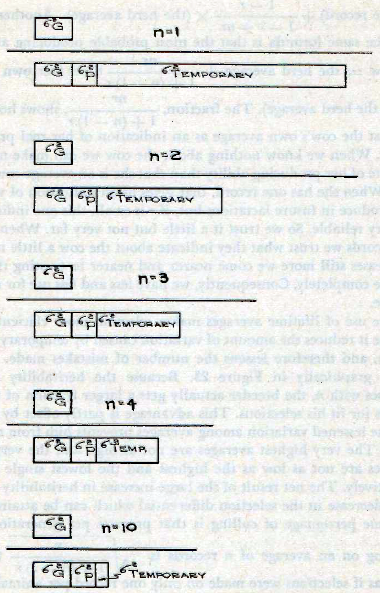
\includegraphics[width=\textwidth]{Figure_23.png}
    \caption{Diagram showing how the heritability of differences between averages
increases as the number ($n$) of records in each average increases. Drawn to scale for
the case in which heritability of differences is .12 when $n$ is 1 and repeatability of
single records is .20. That means the case in which 80 per cent of the variance
between animals with one record each is caused by temporary environmental circumstances.
$\sigma_G^2$ is the additively genetic variance between individuals. $\sigma_P^2$ is the variance
due to permanent but nontransmissible differences between individuals. These
include differences due to dominance deviations, epistatic deviations, and to such
effects of environment as are permanent for each animal but differ from one animal
to another. As $n$ increases, the variance due to temporary things falls to one $n$th of its
value in single records.}
    \label{fig:Lush_Figure_23}
\end{figure}

In records of yearly milk and fat production, considering only cows
which are in the same herd, $r$ is usually somewhere between \nicefrac{1}{3} and
\nicefrac{1}{2}. We shall not be far wrong if we take \nicefrac{2}{5} as the general figure to be
used in the preceding equation, although a higher figure would be justified
in herds where management has been unusually standardized and
corrections for the known environmental circumstances have been
unusually complete. In fact, $r$ is the fraction of the total variance among
the corrected records which is due to permanent differences between
cows; and $1 - r$ is the fraction of the variance caused by temporary circumstances
which vary from one record to another of the same cow.
\index{Variation!of averages|)}

\begin{table}[t]
	\centering
	\caption{\textsc{Progress When Selecting Between Animals With} $n$ 
	\textsc{Records Each, as a Multiple of the Progress Which Could Be Made by
	Selecting Between Them When They Had Only One Record Each}}
	\label{tbl:Lush_Table_13}
	\begin{tabular}{l|c|c|c|c|c|c|c|c|c}
		\hline
		\hline
		 		& \multicolumn{9}{c}{$r$} \\
		 \cline{2-10}
		 $n$	& .1	& .2	& .3	& .4	& .5	& .6	& .7	& .8	& .9 \\
		 \hline
		 2		& 1.35	& 1.29	& 1.24 	& 1.20 	& 1.15	& 1.12	& 1.08	& 1.05 	& 1.03 \\
		 3		& 1.58	& 1.46	& 1.37	& 1.29	& 1.22	& 1.17	& 1.12	& 1.07 	& 1.04 \\
		 4		& 1.75	& 1.58	& 1.45	& 1.35	& 1.26	& 1.20	& 1.14	& 1.08 	& 1.04 \\
		 6		& 2.00	& 1.73	& 1.55	& 1.41	& 1.31	& 1.22	& 1.15	& 1.10 	& 1.04 \\
		 10		& 2.29	& 1.89	& 1.64	& 1.47	& 1.35	& 1.25	& 1.17	& 1.10 	& 1.05 \\
		 \hline
	\end{tabular}
\end{table}

\noindent
More rigid control of the environment will naturally make $r$ higher.
That is, $r$ is a description of conditions in a particular population and
is not a fundamental biological constant. If we use the fraction \nicefrac{2}{5} in
the preceding example, the equation simplifies to: The cow's ability
\(= \dfrac{2n}{2n + 3} \times (\textrm{her own average}) + \dfrac{3}{2n + 3}
\times (\textrm{herd average})\).
That gives the following for estimates of the real producing ability of the three
cows: A = 480 pounds; B = 494 pounds; C = 516 pounds. C is probably
the best and A the poorest of these three, so far as the evidence
goes; but all three are good cows, and the differences between them are
small enough that we should not be greatly surprised if another lactation
or two would change their order.
\index{Environment and heredity|)}
\index{Regression|)}

Figure~\ref{fig:Lush_Figure_24} shows graphically the results of such computations for
butterfat production in an actual herd. The numbers along the vertical
scale are the barn numbers of the cows. Such a graphic scale of estimated
productive ability is a convenient help in making decisions about
culling the cows or saving bull calves from various cows. It must be
kept reasonably up to date, of course, if it is to be useful. At any particular
time some of the cows will have incomplete records which indicate
their producing ability but do not merit as much confidence as completed
records. In making Figure~\ref{fig:Lush_Figure_24}, the records estimated from lactations
still incompleted have arbitrarily been given about half as much
confidence as completed records in the case of cows which have not yet
completed their second record. The incomplete records were not used
at all for other cows. The heifers with only an incomplete lactation were
placed by themselves on the right to emphasize further the uncertainty
about their ability. The cows at the extreme left were included to show
whether those which left the herd either through death, disability, or
voluntary culling, had really averaged less in productive ability than
those which remained.

\begin{figure}[htbp]
	\centering
    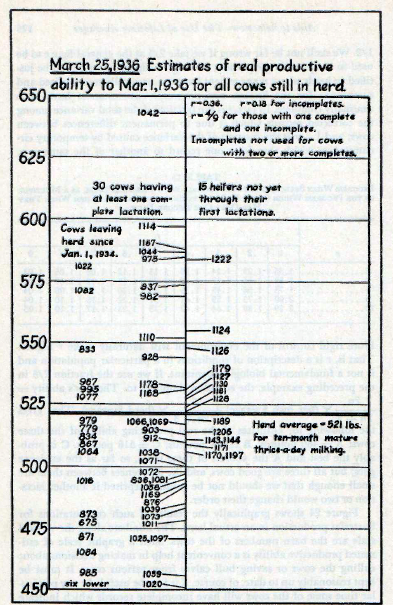
\includegraphics[width=\textwidth]{Figure_24.png}
    \caption{Estimated producing abilities of many cows with unequal numbers of
    		 lactations, based on all information available at the date when the
    		 scale was made.}
    \label{fig:Lush_Figure_24}
\end{figure}

Many other examples of the use of averages might be given. In each
of them it is necessary to know something about the repeatability of the
characteristic. In fertility of swine the repeatability of the number of
pigs born to the same sow in different litters is about one-sixth. In the
weight of fleeces shorn from sheep, the repeatability is about .5 to .6.
The corresponding figure for the fleece weights of Angora goats is about
.4. Some of the earliest studies on repeatability of production records in
farm animals were made on the records of first and second year egg production
in egg-laying contests. Most of those figures were of the order of
.45 to .60. All of these are computed on the basis of records made within
one herd or flock.

The method of averages can be extended to include scores\index{Scoring} or any
other ratings of type which can be expressed numerically. The repeatability
of such type ratings is usually low enough that there would be
a material gain in the accuracy of selections by obtaining and averaging
type ratings of the animal at different times in its life as compared with
relying upon the opinion of one judge, no matter how expert, who saw
the animal only once. The repeatability of type ratings of dairy cows at
intervals of one year was .34 to .55 in the only study\footnote{\textit{Jour.
of Dy. Sci.} 25:45--56, 1942} yet reported. The
opinions which the same judge would hold of the animal if he inspected
it at different times in its life usually vary more than do the opinions of
several judges who might inspect the animal at nearly the same time.
Probably this varies considerably with the class of animal and with the
ages at which the inspections are made.

The method of averaging repeated observations, of course, is limited
to characteristics which can be observed more than once. It cannot be
applied to such things as growth rates , age to sexual maturity, or to
carcass qualities which can be observed only upon slaughter of the
animals. It is also limited in usefulness for egg production, where such
a large part of the total economical lifetime production of the bird is
made during its first year.
\index{Repeatability|)}

Of course the costs of waiting to cull until more records are available
need to be considered, too. Besides the actual loss incurred by
keeping any animal which is not actually paying its way, such waiting
tends to make the interval between generations longer and thereby to
lower the progress \textit{per year}. This will partly offset the gain it makes by
increasing the progress \textit{per generation}. The costs of waiting to cull
would vary with the animal and with economic circumstances, being
higher with hens, for example, where the second year's production is
lower than the first, than with cows where the second record is generally
some 12 to 15 per cent higher than the first.

In the case of cows the first lactation will be several months along
and the heifer may be with calf again before it is certain that the production
in her first lactation will be very low. Often it will not cost
much then to keep her enough longer for the first three or four months
of the second lactation to confirm or disprove what the first lactation
indicated. A practical rule for many herds is to cull in their first lactations
only those with extremely low production, keeping the moderately
low and doubtful ones through the flush of production in their second
lactations. They will usually pay at least their feed costs for that,
since so much of the production comes in the first half of the lactation.

In many cases the decision to keep or cull must be made while the
animals are young if economic loss is to be avoided. For example, with
range cattle or sheep the heifer calves and ewe lambs can usually be
sold to better advantage and with lower feed costs at or soon after weaning
age than if they are kept much longer. The ranchman could cull
them more accurately if he could wait until they grow up and until he
can have rated their type several times, but the gain from doing this
may not be enough to pay for the loss he will take in lower sale prices
for those which are finally culled after they are too old to be sold as
heifer calves or lambs.

\index{Abnormal records|(}One practical problem involved in using lifetime averages is what
to do with records thought to have been made under abnormal conditions
for which no satisfactory correction is known. In principle such
records should be omitted. The practical difficulty is how to decide
fairly when conditions really were abnormal.\index{Abnormal records|)} Some circumstances are
definite enough that they offer no difficulty. For example, in Denmark
records are omitted for years in which the cow aborted or had foot-and-mouth
disease. No other omissions are permitted. Other circumstances
are not definite enough to permit a clear decision. For example, a cow
may have had a bad attack of milk fever at the beginning of her lactation.
The owner may believe that she did not recover soon enough to
produce normally during that lactation. But how is one to be certain?
To base the decision on the size of the record opens the door to all
kinds of biases. The guiding principle should be to omit no record
except when the circumstances are so definite that no doubt can exist.
Those circumstances must be something other than the size of the record
of performance itself.

Basing selections on lifetime averages will automatically foster some
selection for longevity and real ``constitution,'' since breeders will tend
to save for sires only the sons of females which have proved themselves
by several records of production. When selections are based on lifetime
averages, it will hardly be possible for a heifer or gilt with only one
record of production to get her son saved to head a purebred herd
unless that one record was truly phenomenal.

\section*{SUMMARY}

The use of an average of many repeated observations as a basis of
selection is one of the most effective ways of overcoming mistakes and
confusion which would otherwise result from the effects of temporary
environmental conditions. The method is inexpensive, requiring only
the existence of the records, the time needed for averaging them, and
whatever it costs to postpone culling until two or more observations
have been made. It can be made to foster some selection for longevity
and constitution. In using such lifetime averages, allowance must be
made for the lessened variability of averages which are based on many
records. If this is not done, it will appear that most of the extreme producers,
both high and low, are individuals with only one or at most
two records. The method is needed most for things which are least constant
from one time to another in the animal's life. Much of the gain
from using it comes with the second record, but if $r$ is small the gain
from waiting for a third or even a fourth record may be considerable.
The method does not help at all to keep the breeder from being
deceived by permanent effects of environment, such as permanent
stunting when young, nor by the consequences of dominance and complex
gene interactions. Placing much reliance on selecting animals by
their lifetime averages will naturally lead men generally to buy breeding
stock from herds which they know well and in which they have
had several opportunities to study the animals.
\index{Lifetime Averages|)}